\documentclass{article}
\usepackage{amsmath}
\usepackage{tikz}
\usetikzlibrary{knots} % 画扭结辅助宏包


\begin{document}



% 第一个图
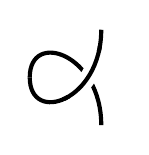
\begin{tikzpicture}[
  x=1ex, y=1ex,
  line width=1.5,
]
\begin{knot}[
    clip width=2,
]
% 自动断开在图片缩小之后有问题,手动断开。
% \strand  (0.6,0.9) .. controls (0.6,0.3) and (0,0.1) .. (0,0.5) .. controls (0,0.9) and (0.6,0.7) .. (0.6,0.1) ;
\strand  (6,9) .. controls (6,3) and (0,1) .. (0,5);
\strand  (0,5) .. controls (0,9) and (6,7) .. (6,1);
\end{knot}
\end{tikzpicture}

\newcommand{\KPa}[0]{%
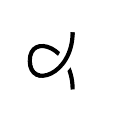
\begin{tikzpicture}[x=1ex, y=1ex, line width=1.5, 
  baseline={([yshift=-.5ex]current bounding box.center)},
  scale=0.6,
]
\begin{knot}[ clip width=2,
  end tolerance=1pt,
]
\strand  (6,9) .. controls (6,3) and (0,1) .. (0,5);
\strand  (0,5) .. controls (0,9) and (6,7) .. (6,1);
\end{knot}
\end{tikzpicture}%
}


% 第二张图 `O|`
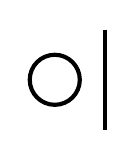
\begin{tikzpicture}[x=1ex,y=1ex,line width=1.5,
  scale=0.6,
]
  \begin{knot}
    \filldraw[fill=none] circle (3.5);
    \strand (7,7) -- (7,-7);
  \end{knot}
\end{tikzpicture}

\newcommand{\KPb}[0]{%
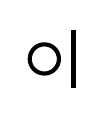
\begin{tikzpicture}[x=1ex,y=1ex,line width=1.5,
  scale=0.35,
  baseline={([yshift=-.5ex]current bounding box.center)},
]
  \begin{knot}
    \filldraw[fill=none] circle (3.5);
    \strand (7,7) -- (7,-7);
  \end{knot}
\end{tikzpicture}%
}


% 第三张图
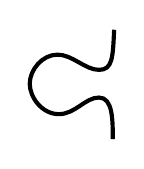
\begin{tikzpicture}[x=0.5pt,y=0.5pt]
  \begin{knot}
    \strand [line width=1.5] (230.51,238.92) .. controls (229.51,218.92) and (229.51,209.92) .. (219.51,209.92) .. controls (209.51,209.92) and (200.51,220.92) .. (189.51,220.92) .. controls (178.51,220.92) and (169.51,209.92) .. (169.51,199.92) .. controls (169.51,189.92) and (178.51,177.92) .. (190.51,177.92) .. controls (202.51,177.92) and (209.51,189.92) .. (219.51,189.92) .. controls (229.51,189.92) and (229.51,173.92) .. (229.51,159.92) ;
  \end{knot}
\end{tikzpicture}

\newcommand{\KPc}[0]{%
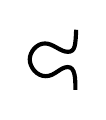
\begin{tikzpicture}[x=0.5pt,y=0.5pt,
  baseline={([yshift=-.5ex]current bounding box.center)}, % 基线对齐
  scale=0.55, % 调整大小
]
  \begin{knot}
    \strand [line width=1.5] (230.51,238.92) .. controls (229.51,218.92) and (229.51,209.92) .. (219.51,209.92) .. controls (209.51,209.92) and (200.51,220.92) .. (189.51,220.92) .. controls (178.51,220.92) and (169.51,209.92) .. (169.51,199.92) .. controls (169.51,189.92) and (178.51,177.92) .. (190.51,177.92) .. controls (202.51,177.92) and (209.51,189.92) .. (219.51,189.92) .. controls (229.51,189.92) and (229.51,173.92) .. (229.51,159.92) ;
\end{knot}
\end{tikzpicture}%
}

% 第四张图 `|`
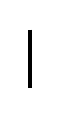
\begin{tikzpicture}[x=1ex,y=1ex,line width=1.5,
  scale=0.35,
  baseline={([yshift=-.5ex]current bounding box.center)},
]
  \begin{knot}
    \strand (0,7) -- (0,-7);
  \end{knot}
\end{tikzpicture}

\newcommand{\KPd}[0]{%
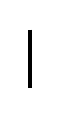
\begin{tikzpicture}[x=1ex,y=1ex,line width=1.5,
  scale=0.35,
  baseline={([yshift=-.5ex]current bounding box.center)},
]
  \begin{knot}
    \strand (0,7) -- (0,-7);
  \end{knot}
\end{tikzpicture}%
}


A path consists of a series of lines and Bézier cubics. The “explosion” of a path
uses this decomposition. Unfortunately, even that is not always enough as it is
possible for a Bézier cubic to self-intersect. The consider self intersections
also splits these Bézier curves in two to ensure that this doesn’t happen1
. To
disable this, use the consider self intersections=no splits option. This is
the recommended option.

\begin{equation} \label{eq1}
\begin{split}
\left\langle \ \KPa \right\rangle 
  & = A \left\langle \KPb \ \right\rangle
    + B \left\langle \KPc \  \right\rangle \\
  & = Ad \left\langle \ \  \KPd \ \  \right\rangle 
    + B \left\langle \ \  \KPd \ \  \right\rangle \\
  & = (Ad + B) \left\langle \ \  \KPd \ \  \right\rangle \\
\end{split}
\end{equation}


The clip width=<factor> is the multiplier for the thickness of the “wipeout” path relative to the line width of the actual path.

\end{document}